\documentclass[12pt, letterpaper]{article}

\title{
  CSE 3241 Project Checkpoint 2\\
  \large{Relational Model and Relational Algebra}
}
\author{Wally Yang, Tina Liang, Wei Zong, Chuwen Sun, Xingyu Yan}
\date{\today}

\usepackage[margin=1in]{geometry}

\usepackage{amsmath}
\setlength{\jot}{12pt} % set the vertical spacing between lines

\usepackage{listings}
\usepackage{xcolor}

\definecolor{codegreen}{rgb}{0,0.6,0}
\definecolor{codegray}{rgb}{0.5,0.5,0.5}
\definecolor{codepurple}{rgb}{0.58,0,0.82}
\definecolor{backcolour}{rgb}{0.95,0.95,0.92}

\lstdefinestyle{mystyle}{
  backgroundcolor=\color{backcolour},
  commentstyle=\color{codegreen},
  keywordstyle=\color{magenta},
  numberstyle=\color{codegray},
  stringstyle=\color{codepurple},
  basicstyle=\ttfamily\footnotesize,
  breakatwhitespace=false,
  breaklines=true,
  captionpos=b,
  numbers=left,
  numbersep=5pt,
  showspaces=false,
  showstringspaces=false,
  showtabs=false,
  gobble=10,
  tabsize=2
}
\lstset{style=mystyle}

\usepackage{amssymb}
\def\ojoin{\setbox0=\hbox{$\bowtie$}%
  \rule[-.02ex]{.25em}{.4pt}\llap{\rule[\ht0]{.25em}{.4pt}}}
\def\leftouterjoin{\mathbin{\ojoin\mkern-5.8mu\bowtie}}
\def\rightouterjoin{\mathbin{\bowtie\mkern-5.8mu\ojoin}}
\def\fullouterjoin{\mathbin{\ojoin\mkern-5.8mu\bowtie\mkern-5.8mu\ojoin}}

\usepackage{graphicx}
% \graphicspath{ {./images/} }

\begin{document}
\maketitle

\begin{enumerate}

\item Updated ER Model
  \begin{center}
    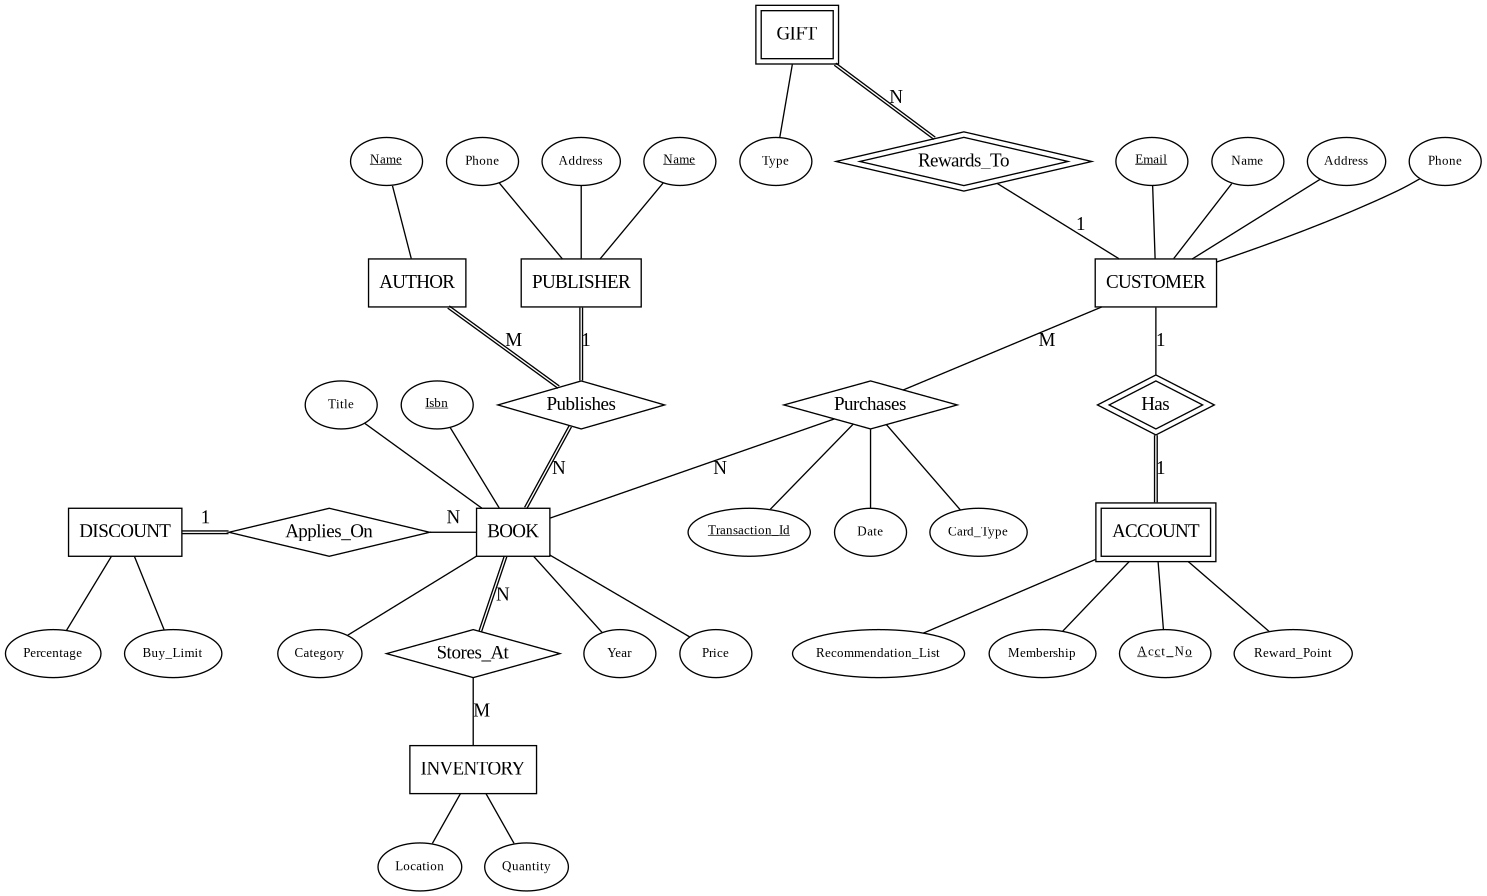
\includegraphics[width=\linewidth]{cp2.png}
  \end{center}

  \pagebreak

\item Relational Schema
  \begin{center}
    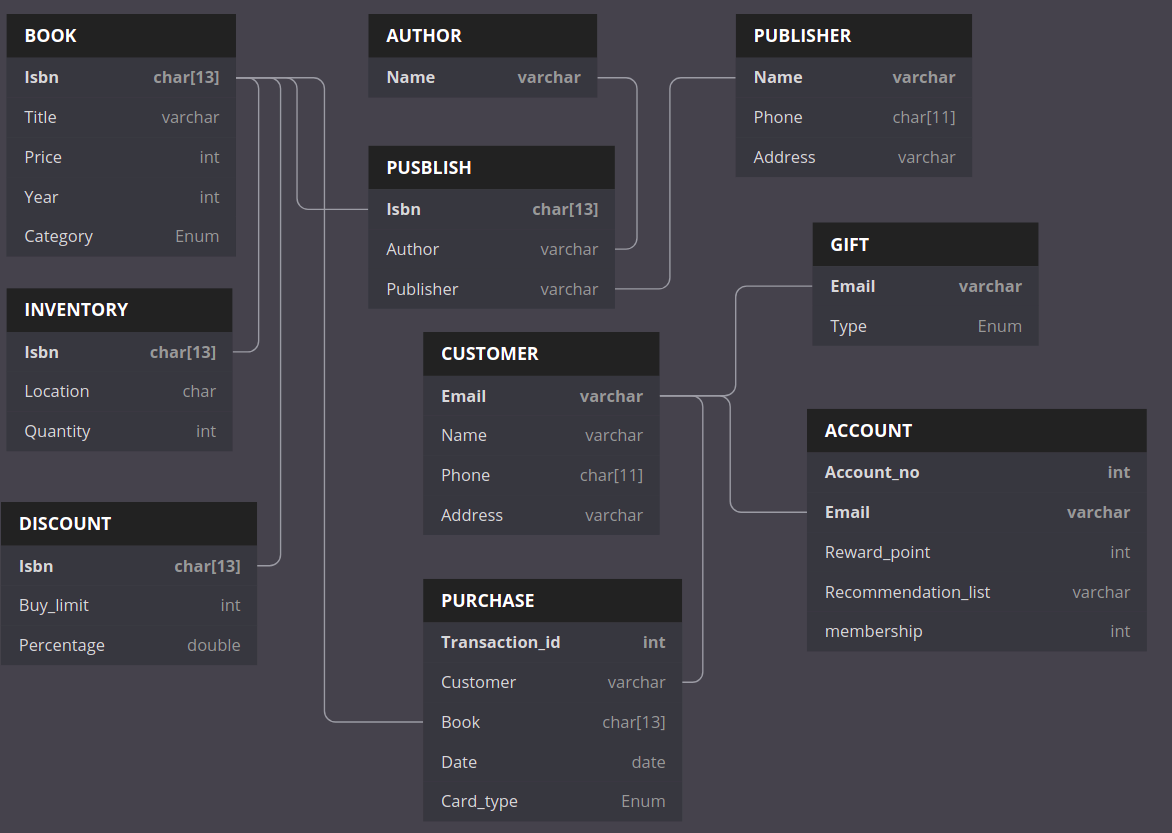
\includegraphics[width=\linewidth]{RS.png}
  \end{center}

\item
  \begin{enumerate}

  \item Find the titles of all books by Pratchett that cost less than \$10
    \begin{equation*}
      \pi_{\textit{Title}}(\sigma_{\textit{Price} < 10}(BOOK))
    \end{equation*}

  \item Give all the titles and their dates of purchase made by a single
    customer (you choose how to designate the customer)\\
    designate CUSTOMER with Email
    \begin{align*}
      &\textit{BOOKS} \leftarrow \textit{BOOK} \bowtie_{\textit{Isbn} = \textit{Book}} (\sigma_{\textit{Customer}=\textit{Email}}(\textit{PURCHASE}))\\
      &\textit{RESULT} \leftarrow \pi_{Title, Date} (\textit{BOOK})
    \end{align*}

  \item Find the titles and ISBNs for all books with less than 5 copies in stock
    \begin{align*}
      &\textit{STOCK(Isbn, Quantity)} \leftarrow _{\textit{Isbn}}\mathcal{F}_{\textit{SUM Quantity}}(\textit{INVENTORY})\\
      &\textit{RESULT} \leftarrow \pi_{\textit{Title}, \textit{Isbn}}(\sigma_{\textit{Quantity} < 5}(STOCK))
    \end{align*}

  \item Give all the customers who purchased a book by Pratchett and the titles of Pratchett books they purchased
    \begin{align*}
      &\textit{PRATCHETTS} \leftarrow (\sigma_{\textit{Author} = \textit{Pratchett}}(\textit{PUBLISH}) * \textit{BOOK})\\
      &\textit{SALES} \leftarrow (\textit{PRATCHETTS} * \textit{PURCHASE})\\
      &\textit{RESULT} \leftarrow (\pi_{\textit{Email}, \textit{Name}, \textit{Title}}(\textit{SALES}))
    \end{align*}

  \item Find the total number of books purchased by a single customer (you choose how to designate the customer)
    \begin{align*}
      &\textit{COUNT(Customer, \# of Books)} \leftarrow _{\textit{Customer}}\mathcal{F}_{\textit{COUNT BOOK}}(\textit{PURCHASE})\\
      &\textit{RESULT} \leftarrow \sigma_{\textit{Customer} = \textit{Email}}(\textit{COUNT})
    \end{align*}

  \item Find the customer who has purchased the most books and the total number of books they have purchased
    \begin{align*}
      &\textit{COUNT(Customer, No)} \leftarrow _{\textit{Customer}}\mathcal{F}_{\textit{COUNT BOOK}}(\textit{PURCHASE})\\
      &\textit{RESULT} \leftarrow _{\textit{Customer}}\mathcal{F}_{\textit{MAX No}}(\textit{COUNT})
    \end{align*}

  \end{enumerate}

  \item
    \begin{enumerate}

    \item Find the CUSTOMER with the most Reward\_point on his/her account
    \begin{align*}
      &\textit{CACCT} \leftarrow \textit{CUSTOMER} * \textit{ACCOUNT}\\
      &\textit{RESULT} \leftarrow \pi_{\textit{Email, Name}}(_{\textit{Email, Name}}\mathcal{F}_{\textit{MAX Reward\_point}}(\textit{CACCT}))
    \end{align*}

  \item Find the most expensive BOOK with all the DISCOUNT applied
    \begin{align*}
      &\textit{DIS\_BOOKS} \leftarrow \textit{BOOK} \leftouterjoin \textit{DISCOUNT}\\
      &\textit{RESULT} \leftarrow _{\textit{Isbn, Title}}\mathcal{F}_{\textit{MAX} (\textit{Price} * \textit{percentage})}(\textit{DIS\_BOOKS})
    \end{align*}

  \item Find the total price of all the BOOK for each stock (quantity * price)
    \begin{align*}
      &\textit{STOCK} \leftarrow \textit{BOOK} * _{\textit{Isbn}}\mathcal{F}_{\textit{SUM Quantity}}(\textit{INVENTORY})\\
      &\textit{RESULT} \leftarrow \pi_{\textit{Isbn}, \textit{Quantity * Price}}(\textit{STOCK})
    \end{align*}

    \end{enumerate}

\end{enumerate}

\end{document}